


\documentclass{article}[12pt]
\usepackage{fullpage,graphicx, setspace, latexsym, cite,amsmath,amssymb,color,subfigure}
%\usepackage{epstopdf}
%\DeclareGraphicsExtensions{.pdf,.eps,.png,.jpg,.mps} 
\usepackage{amssymb} %maths
\usepackage{amsmath} %maths
\usepackage{amsthm}
\usepackage[ruled,vlined]{algorithm2e}

\bibliographystyle{unsrt}

\newtheorem{theorem}{Theorem}
\newtheorem{prop}{Proposition}
\newtheorem{corollary}{Corollary}
\newtheorem{lemma}{Lemma}
\newtheorem{defn}{Definition}
\newtheorem{ex}{Example}
\usepackage{float}

\def\R{\mathbb{R}}
\def\Eps{\mathcal{E}}
\def\E{\mathbb{E}}
\def\V{\mathbb{V}}
\def\F{\mathcal{F}}
\def\G{\mathcal{G}}
\def\H{\mathcal{H}}
\def\S{\mathcal{S}}
\def\P{\mathbb{P}}
\def\1{\mathbf{1}}
\def\n{\nappa}
\def\h{\mathbf{w}}
\def\v{\mathbf{v}}
\def\x{\mathbf{x}}
\def\X{\mathcal{X}}
\def\Y{\mathcal{Y}}
\def\eps{\epsilon}
\def\y{\mathbf{y}}
\def\e{\mathbf{e}}
\newcommand{\norm}[1]{\left|\left|#1\right|\right|}
\DeclareMathOperator*{\argmin}{arg\,min}
\DeclareMathOperator*{\argmax}{arg\,max}

\newcommand{\lecture}[4]{
   \pagestyle{myheadings}
   \thispagestyle{plain}
   \newpage
   % \setcounter{lecnum}{#1}
   \setcounter{page}{1}
   \setlength{\headsep}{10mm}
   \noindent
   \begin{center}
   \framebox{
      \vbox{\vspace{2mm}
    \hbox to 6.28in { {\bf ESE 680-004: Learning and Control
   \hfill Fall 2019} }
       \vspace{4mm}
       \hbox to 6.28in { {\Large \hfill Lecture #1: #2  \hfill} }
       \vspace{2mm}
       \hbox to 6.28in { {\it Lecturer: #3 \hfill Scribes: #4} }
      \vspace{2mm}}
   }
   \end{center}
   \markboth{Lecture #1: #2}{Lecture #1: #2}

   \noindent{\bf Disclaimer}: {\it These notes have not been subjected to the
   usual scrutiny reserved for formal publications. }
   \vspace*{4mm}
}

%notation

\def \E{\mathbb E}
\def \P{\mathbb P}
\def \R{\mathbb R}
\def \A{\cal A}

\begin{document}

\lecture{20}{Model Free Methods 3}{Nikolai Matni}{Walker Gosrich}

\section{Introduction}
So far in the class, we have looked at several methods for solving reinforcement learning problems, including model-based and model-free approaches. Here, we will continue our discussion of model-free approaches, by considering \textit{direct policy search.} 

First, we'll look at Section 3.3 of \cite{Recht2019} for a discussion of direct policy search and an introduction to the REINFORCE algorithm, a simple and highly versatile algorithm for derivative-free (function evaluation-based) optimization of unconstrained problems. We'll also be introduced to Policy Gradient and Pure Random Search methods, from Section 4 of the same. Then we'll briefly see how these approaches compare, applied to a simple test case: the LQR.

After this, we'll turn to \cite{Fazel2018} for a look at the theoretical properties and the ``optimization landscape'' of model-free methods applied to LQR. We'll analyze both the model-based and model-free cases of this problem, prove convergence to the optimal policy, and characterize the sample-complexity of this convergence.

\section{REINFORCE Algorithm}
First, we'll develop a simple and very general algorithm, typically called REINFORCE, that is used to solve unconstrained optimization problems through function evaluations. 

Let's begin by considering the generic unconstrained optimization problem:

\begin{equation}
\text{minimize}_{c \in \R_d}C(z) 
\end{equation}

where we aim to find the value of $z$ that minimizes our cost function. We claim that the problem of finding the minimizing value of $z$ is equivalent to the problem of finding the minimizing \textit{probability distribution} over $z$:

$$\text{minimize}_{p(z)}\E_p \left[C(z)\right]$$

If $z^*$ is the minimizing argument of $C(z)$, then we can do at least as well by choosing a probability distribution: we can achieve the same value of $C(z)$ by choosing the $\delta$-function around $z^*$. 

Furthermore, we can do no better than a fixed policy by applying a probability distribution. To see this, note that for a fixed dsitribution $p$, we must have $\E_p[C(z)]\geq \text{min}_zC(z)$. Because $p$ is an arbitrary distribtion, we know that $\text{min}_p\E_p[C(z)]\geq \text{min}_zC(z)$ also holds. So we can do at least as well as our fixed value, and can do no better: the two problems are equivalent, and we can choose: optimize over $z$ or \textit{distributions} of $z$.

The space of distributions over $z$ is infinite-dimensional, so we typically restrict ourselves to a subset of the space that we can efficiently optimize over. A typical approach is to parameterize by a vector $\theta$, considering the family of density functions $p(z;\theta)$. We now have the following problem:

\begin{equation}
\text{minimize}_\theta \E_{p(z;\theta)}[C(z)]
\end{equation}

Note that by restricting ourselves to this family of probability density functions, we have upper-bounded our performance on the problem. Our parameterization may contain all of the $\delta$-functions, in which case we could reach the same performance as the original optimization. But our family of distributions will likely not contain all $\delta$-functions, and so we will likely perform sub-optimally.

But our reformulation has a purpose. Now, we can compute the derivative of $\E_{p(z;\theta}[C(z)]$ using a method called the \textit{log likelihood trick.} We define the cost $J(\theta):=\E_{p(z;\theta)}[C(z)]$, and examine  the derivative with respect to $\theta$: $\nabla_\theta J(\theta)$. We perform the following manipulation:

\begin{align*}
\nabla_\theta J(\theta) &= \int C(z) \nabla_\theta p(z;\theta)dz\\
&= \int C(z) \frac{\nabla_\theta p(z;\theta)}{p(z;\theta)}p(z;\theta)dz\\
&= \int [C(z)\nabla_\theta \text{log }p(z;\theta)]p(z;\theta)dz\\
&= \E_{p(z;\theta)}[C(z)\nabla_\theta \text{log }p(z;\theta)]
\end{align*}

This tells us that the gradient of $J(\theta)$ is the expected value of the function 

\begin{equation}
G(z,\theta) = C(z)\nabla_\theta \text{log }p(z;\theta)
\end{equation}

We can sample $z$ from $p(z;\theta)$, and evaluate the function $G(z,\theta)$ to give us an unbiased estimate of the gradient of $J(\theta)$. Using these function evaluations, we can follow the gradient and perform stochastic gradient descent on $J(\theta)$. This approach gives us the REINFORCE algorithm \cite{Willia1992} - Algorithm 1.

\begin{algorithm}[H]
\SetAlgoLined
\textbf{Hyperparameters:} step sizes $\alpha_j > 0 $\\
\textbf{Initialize:} $\theta_0,k = 0$\;
 \While{ending condition not satisfied}{
  sample $z_k \sim p(z;\theta_k)$\;
  set $\theta_{k+1} \leftarrow \theta_k - \alpha_kC(z_k)\nabla_\theta \text{log } p(z_k;\theta_k)$ \;
  $ k \leftarrow k + 1$ \;
  }
 \caption{REINFORCE}
\end{algorithm}

The main benefit of Algorithm 1 is that it is incredible simple to implement. If you can sample efficiently from $p(z;\theta)$, then you can run the algorithm on essentially any problem. However, this generality comes at a cost: we now only access our cost function $C(z)$ through function evaluations. Because we've used the log-likelihood trick, we are using a derivative-free optimization method, and can not achieve the same performance as methods that compute actual gradients. This performance gap is exacerbated when the function evaluations are noisy. Another drawback to this approach is that our choice of probability distribution can lead to high variance of stochastic gradients. High variance requires more samples to be drawn in order to find a minima or maxima. In other words, sample complexity increases.

Although the approach has a few drawbacks, the simplicity of implementation is often valuable enough to justify its use. There are two primary applications of this sort of stochastic search approach in reinforcement learning: policy gradient and pure random search.

\section{Policy Gradient}
In reinforcement learning, our goal is typically to minimize some cost (or conversely, maximize a reward subject to system dynamics. This is stated as follows:

\begin{equation}
\text{minimize }  \E \left[ \sum_{t=0}^N C_t(x_t,u_t)\right]\\
\text{subject to } x_{t+1} = f_t(x_t,u_t,e_t)
\end{equation}

We can see from Bellman's equation that the optimal policy for the above problem is always deterministic. However, for policy gradient, we relax our search to probabilistic policies. This isn't too unreasonable: these policies are optimal for other sorts of problems, such as MDPs or zero-sum games.

Let's consider parametric, randomized policies such that $u_t$ is sampled from a distribution $p(u|\tau_t;\theta)$, where $\tau_t = \{x_{0:t},u_{0:t-1}\}$, the observed trajectory up to time $t$. This probabilistic policy induces a probability distribution over trajectories:

$$p(\tau;\theta) = \prod_{t=0}^{N-1}p(x_{t+1}|x_t;u_t)p(u_t|\tau_t;\theta)$$

Further, if we overload notation, and define the cost over a trajectory as follows:

$$C(\tau) = \sum_{t=0}^{N-1}C(x_t,u_t)$$

then we can write Equation 4 as the following optimal control problem:

\begin{equation}
\text{minimize}_\theta \E_{p(\tau;\theta)}[C(\tau)]
\end{equation}

which is identical to Equation 2! Policy gradient proceeds by sampling a trajectory using the probabilistic policy, and updating using REINFORCE to find the solution.

We can verify that the gradient of $J(\theta) = \E_{p(\tau,\theta)}[C(\tau)]$ is not an explicit function of the dynamics:

\begin{align*}
\nabla_\theta J(\theta) &= \E_{p(\tau;\theta)}[C(\tau)\nabla_\theta\text{log }p(\tau;\theta)]\\
&= \E_{p(\tau;\theta)}[C(\tau)\nabla_\theta\left[\sum_{t=0}^{N-1}\text{log }p(x_{t+1}|x_t,u_t)+\sum_{t=0}^{N-1}\text{log }p(u_t|\tau_t;\theta)\right]\\
&=\sum_{t=0}^{N-1}\E_{p(\tau;\theta)}[C(\tau)\nabla_\theta\text{log }p(u_t|\tau_t;\theta)]
\end{align*}

This expectation can then be approximated by applying REINFORCE. This should not be surprising though: by shifting to distribution over policies, we push the burden of optimization onto the sampling procedure.

\section{Pure Random Search}
An older and more widely applied approach to solve Equation 1 is to directly perturb the current decision variable $z$ with random noise, and then update the model based on the received reward at this perturbed value. Again, we can apply the REINFORCE algorithm without any knowledge of the underlying dynamics. In effect, applying reinforce is equivalent to approximate gradient descent of $C(z)$. We consider drawing random perturbations $\epsilon$ according to some distribution - most simply a uniform or normal distribution. We compute the following approximate gradient step update:

$$\theta_{t+1} = \theta_t -\alpha g_\sigma(\theta_t)$$

where 

$$g_\sigma (\theta) = \frac{C(\theta + \sigma \epsilon) - C(\theta - \sigma \epsilon)}{2 \sigma}\epsilon$$
is a finite difference approximation to the gradient along direction $\epsilon$. So this approach steps along the gradient in direction $\epsilon$. We can reduce the variance of these gradient estimates by averaging over multiple random directions:

$$g_\sigma^{(m)} = \frac{1}{m}\sum_{i = 1}^m \frac{C(\theta + \sigma \epsilon_i) - C(\theta - \sigma \epsilon_i)}{2 \sigma}\epsilon_i$$

The pure random search method is simpler to implement than the policy search method, but uses less of the structure of the problem. It is difficult to say which approach is better without selecting a specific problem to which to apply them. In the next section, we'll look at how these algorithms perform on linear quadratic regulator problems. 

\textbf{Side note:} in \cite{Mania2018}, Mania, Guy, and Recht used a pure random search of static linear policies to take on some of the benchmarks in OpenAI Gym. They managed to beat the state of the art, using orders of magnitude less training data. The (intended) takeaway is that these benchmark tasks in OpenAI Gym and other environments aren't all that hard - after all, one of the simplest canonical algorithms can perform really well! But a lot of the field had a different takeaway: we should be using more of random search and linear policies! 

\section{Application to LQR}
To compare the above approaches, let's take a look at the simplest nontrivial problem that can help distinguish between them. In control, this is the linear quadratic regulator: linear dynamics, and convex rewards/costs. In fact, let's start with an even simpler example with no dynamics:

$$\text{minimize }C(u) = ||u||_2^2 \text{, for }u\in \R^d$$

Applying policy gradient, we parameterize our policy as 
$$p(u;\theta) = \mathcal{N}(\theta,\sigma^2 I)$$
Then we can evaluate the formula in Equation 2:
$$\E_{p(u;\theta)}[C(u)] = ||\theta||_2^2+\sigma^2d$$
As we are simply minimizing the square of the norm of our input, the best place to start is clearly $\theta_* = 0$. This will still leave us $\sigma^2d$ off from optimal, but it will give us a good starting guess.

As a function of $\theta$, the cost is strongly convex. Also, from what we've seen in our analysis of stochastic gradient descent, we need bounds on the (expected) norm of the gradient. If we draw $u \sim \mathcal{N}(\theta_0,\sigma^2 I)$, we can compute $G(u,\theta_0)$, our approximate gradient from Equation 3.

$$G(u,\theta) =  C(u)\nabla_\theta\text{log } p(u;\theta) = - \frac{||w-\theta_0||_2^2w}{\sigma^2}, w\sim\mathcal{N}(0,\sigma^2I)$$

We can show that the expected norm of this gradient scales as $O(\sigma d^{3/2} + \frac{d^{1/2}||\theta_0||_2}{\sigma})$, a non-trivial scaling with dimension. Interestingly, most bounds analyzing the convergence of these methods scale with the largest magnitude that the cost function can possible take. If you start with a cost function taking values in [0,1] and add $10^6$, the running time may increase by $10^6$, even though you haven't fundamentally changed the problem.

As another case, let's take a look at the classic problem of a discrete-time double integrator with the dynamical model 

\[
x_{t+1} = 
\begin{bmatrix}
1 & 1 \\ 
0 & 1
\end{bmatrix}
x_t + 
\begin{bmatrix}
0\\ 
1
\end{bmatrix}
u_t
\]

Such a system could model the position (first state) and velocity (second state) of a unit mass object under force $u$.
As an instance of LQR, we can try to steer this system to reach point - from initial condition $x_0 = [-1,0]$ without expending much force:

\[Q = 
\begin{bmatrix}
1 & 0 \\ 
0 & 0
\end{bmatrix}
, R = r_0
\]

for some scalar $r_0$. Even in this simple case, there is an element of control design: changing $r_0$ changes the character of the control law, balancing control energy against time required to reach the destination.

To compare the different approaches, the author of \cite{Recht2019} ran experiments on this instance with a small amount of noise ($e_t$ zero mean with covariance $10^{-4}I$) and training episode length $L = 10$. The goal was to design a controller that works on an arbitrarily long time horizon using the fewest number of simulations of length L.

To compare with policy search, the author restricts to policies that use a static, linear gain, as would be optimal on an infinite time horizon. The author used the Adam algorithm to shape the iterates, and subtracted the mean reward of previous iterates, a popular baseline subtraction heuristic to reduce variance. Without these algorithmic changes, the author was unable to get policy gradient to converge.

Figure 1 from \cite{Recht2019} is reproduced here, showing the results from this experiment.

\begin{figure}
\begin{center}
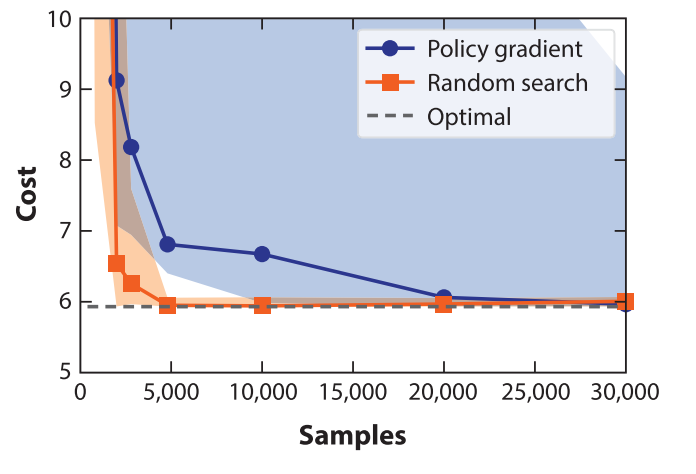
\includegraphics[width = 0.6\linewidth]{fig1}
\caption{Cost for the double-integrator model for various reinforcement learning algorithms. The solid plots denote the median performance, and the shaded regions capture the maximum and minimum performance.}
\end{center}
\end{figure}

\begin{figure}[H]
\begin{center}
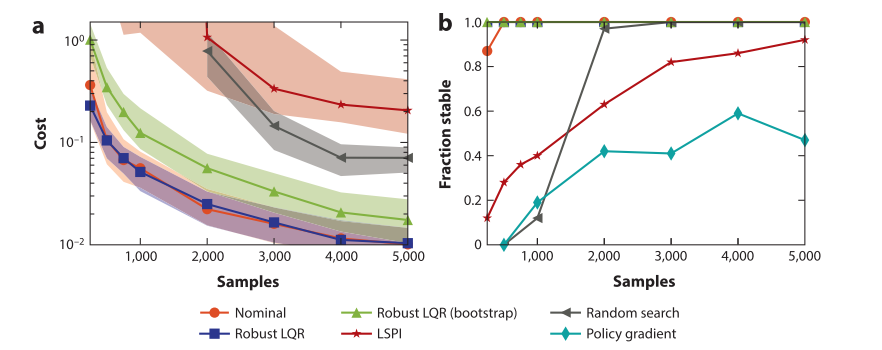
\includegraphics[width = 0.9\linewidth]{fig2}
\caption{(a) Cost for the Laplacian model for varied models over 5,000 iterations. (b) The fraction of the time that the synthesized control strategy returns a stabilizing controller. Abbreviations: LQR, linear quadratic regulator; LSPI, least squares policy iteration}
\end{center}
\end{figure}


The author of \cite{Recht2019} also considered a more complex instance of LQR: unstable Laplacian dynamics. An idealized instance of data canter cooling, a popular application of RL, with three heat sources and cooling devices, is modeled by the following linear dynamical system:

\[
x_{t+1} = 
\begin{bmatrix}
1.01 & 1.01 & 0 \\ 
0.01 & 1.01 & 0.01 \\
0 & 0.01 & 0.01
\end{bmatrix}
x_t + 
\begin{bmatrix}
1 & 0 & 0\\
0 & 1 & 0\\ 
0 & 0 & 1
\end{bmatrix}
u_t + w_t
\]

The LQR problem is approached with settings $Q=I$ and $R = 1,000I$. Figure 3 from \cite{Recht2019} is reproduced here showing the results of applying model-free and model-based methods to learn a solution to this LQR problem. 


\section{Theoretical Properties: Policy Gradient for LQR}

Now, we turn to \cite{Fazel2018} for an in-depth theoretical analysis of the performance of policy gradient methods on an infinite-horizon LQR problem. They consider the following problem:
\begin{equation}
\text{minimize } \E \left[ \sum_{t=0}^\infty (x_t^TQx_t + u_t^TRu_t)\right]
\text{such that } x_{t+1} = Ax_t + Bu_t, x_0 \sim \mathcal{D}
\end{equation}

and make a few important contributions. First, they show that gradient descent on linear policies $u_t = Kx_t$ globally converges to optimal policies, and does so efficiently. Secondly, they showed that simulated trajectories can be used in a stochastic policy gradient method with provable convergence to a globally optimal policy with polynomial computational and sample complexity. And finally, they show that natural policy gradient methods (and their stochastic counterparts) enjoy significantly improved convergence rates.

\subsection{Setup}
In this work, direct policy gradient methods are characterized, where the policy is linearly parameterized by a matrix $K$, such that the controls $u_t = -Kx_t$ are generated. The cost of this policy $K$ is denoted as follows:

\begin{equation}
C(K) := \E_{x_0 \sim \mathcal{D}} \left[ \sum_{t=0}^\infty (x_t^TQx_t + u_t^TRu_t)\right]
\end{equation}

where $\{x_t,u_t\}$ is the trajectory and control sequence resulting from following $K$, starting from $x_0$.

Gradient descent updates the policy, following the update rule:

$$ K \leftarrow K - \eta \nabla C(K)$$

We can more clearly write the gradient in its functional form. With $P_K$ as the solution to

$$P_K = Q + K^TRK + (A-BK)^TP_K(A-BK)$$

we can write 

$$C(K) = \E_{x_0 \sim \mathcal{D}} \left[x_0^TP_Kx_0\right]$$.

Also, define $\Sigma_K$ as the state correlation matrix:

$$\Sigma_K = \E_{x_0 \sim \mathcal{D}} \sum_{t=0}^\infty x_tx_t^T$$.

Now, we can write the gradient in its functional form:

\begin{lemma} (Policy Gradient Expression):

$$\nabla C(K) = 2\left((R+B^TP_KB)K-B^TP_KA\right)\Sigma_K$$

for simplicity later, define:

$$E_K := \left((R+B^TP_KB)K-B^TP_KA\right)$$

so we have $\nabla C(K) = 2E_K\Sigma_K$

\label{lemma1}
\end{lemma}

\textit{Proof:}
The full proof can be found in \cite{Fazel2018}


\subsection{Optimization Landscape}

\begin{lemma} (Gradient Domination)
\label{gradlemma}
Let $K^*$ be an optimal policy. Suppose $K$ has finite cost and $\sigma_{min}(\Sigma+K)>0$. It holds that:

$$ C(K)- C(K^*) \leq \frac{||\Sigma_{K^*}||}{\sigma_{min}(\Sigma+K)^2\sigma_{min}(R)}||\nabla C(K)||_F^2$$
\end{lemma}

\textit{Proof:} comes from analyzing the advantage of the optimal policy $\Sigma^*$ over $\Sigma$ in each step. 

\begin{corollary} (Stationary point characterization)
If $\nabla C(K) = 0$, then either $K$ is an optimal policy or $\Sigma_K$ is rank deficient.
\end{corollary}
Note that $\Sigma_K \geq \Sigma_0 := \E_{x_0 \sim \mathcal{D}}x_0x_0^T$. So if $ \E_{x_0 \sim \mathcal{D}}x_0x_0^T$ is full rank, then $\Sigma_K$ is full rank, and we know that all stationary points are global optima (i.e. $K$ is optimal).

Using the fact that $\Sigma_K \geq \Sigma_0$, we can prove the convergence of $C(K)$ by showing that it is gradient dominated, meaning in this case that $\exists \lambda \text{ s.t. } C(K)-C(K^*) \leq \lambda ||\nabla C(K)||^2$. Proving convergence this way dates back to the 60s with \cite{Polyak1963}, and requires $C(K)$ to be gradient dominated \textbf{and smooth.} If this were the case, we would be able to immediately imply global convergence at a linear rate. However, our cost function is not smooth. Near the boundary between stable and unstable policies, our cost may go from convergent to $\infty$. In other words, we may have $C(K)-C(K+\epsilon) = \infty$. To solve this problem, we observe that as long as we aren't too close to the boundary, the cost function satisfies an "almost smoothness" condition:

\begin{lemma} ("Almost" smoothness) $C(K)$ satisfies:
\label{almostsmoothness}

$$C(K') - C(K) = -2Tr(\Sigma_{K'}(K-K')^TE_K) + Tr(\Sigma_{K'}(K-K')^T(R+B^TP_KB)(K-K'))$$

where $E_K$ here is as defined in Lemma \ref{lemma1}.

\end{lemma}

To see why this helps, consider when $K'$ is sufficiently close to $K$ such that $\Sigma_{K'}\approx \Sigma_K + O(||K-K'||_F)$. Then, considering the order with respect to $(K-K')$, Lemma 3 simplifies as follows:
\begin{align*}
-2Tr(\Sigma_{K'}(K-K')^TE_K) + O(||K-K'||_F^2)\\
= -Tr(K-K')^T2E_K\Sigma_K + O(||K-K'||_F^2)\\
= -Tr(K-K')^T\nabla C(K) + O(||K-K'||_F^2)
\end{align*}

This tells us that as long as small perturbations of the controller lead to small perturbations of the steady state covariance, the cost function admits a Taylor series approximation

$$C(K') - C(K) \approx \langle K - K', \nabla C(K) \rangle + O(||K-K'||_F^2)$$

Quantifying this well-behaved (i.e. smooth) first order Taylor series approximation is used to show that gradient descent converges to critical points. This, combined with a gradient-dominated cost function, is sufficient to conclude convergence to a globally optimal solution despite a non-convex landscape.

\subsection{Main Results}
First, results on exact gradient methods are provided. We'll work through these, establishing global convergence, and then consider model-free methods.

\subsubsection{Model-Based Methods}

We'll use three exact update rules. The gradient descent update is:

$$K_{n+1} = K_n -\eta \nabla C(K_n),$$

the natural gradient descent update is:

$$K_{n+1} = K_n -\eta \nabla C(K_n)\Sigma_{K_n}^{-1},$$

and the Gauss-Newton method update is:

$$K_{n+1} = K_n -\eta (R+B^TP_{K_n}B)^{-1}\nabla C(K_n)\Sigma_{K_n}^{-1}.$$

\begin{theorem} (Global Convergence of Gradient Methods) \\
Suppose $C(K_0)$ is finite and $\mu = \sigma_{min}(\E_{x_0\sim \mathcal{D}}[x_0x_0^T])>0$\\
With the following step sizes and lower bounds for $N$, we have that $C(K_N) - C(K_*)\leq \epsilon$\\
\\
\textbf{Gauss-Newton:} 
$$\eta = 1, \; \; \;N \geq \frac{||\Sigma_{K_*}||_2}{\mu}\text{log}\frac{C(K_0)-C(K_*)}{\epsilon}$$
\\
\textbf{Natural Gradient Descent:} 
$$\eta = \frac{1}{||R|| + \frac{||B||^2C(K_0)}{\mu}}, \; \; \; N \geq \frac{||\Sigma_{K_*}||_2}{\mu}\text{log}\frac{C(K_0)-C(K_*)}{\epsilon} \left(\frac{||R||}{\sigma_{min}(R)}+\frac{||B||^2C(K_0)}{\mu \sigma_{min}(R)}\right)$$
\\
\textbf{Gradient Descent:} for an appropriate (constant) setting of the stepsize $\eta$,
$$\eta = \text{poly}\left(\frac{\mu \sigma_{min}(Q)}{C(K_0)},\frac{1}{||A||_2},\frac{1}{||B||_2},\frac{1}{||R||_2},\sigma_{min}(R)\right)$$
$$N \geq \frac{||\Sigma_{K_*}||_2}{\mu}\text{log}\frac{C(K_0)-C(K_*)}{\epsilon} \text{poly}\left(\frac{C(K_0)}{\mu \sigma_{min}(R)},||A||_2,||B||_2,||R||_2,\frac{1}{\sigma_{min}(R)}\right)$$
\end{theorem}

\textit{Proof:}Gauss-Newton reproduced here, others see supplemental material of \cite{Fazel2018}.

\begin{lemma} First, let

$$K' = K - \eta(R+B^TP_KB)^{-1}\nabla C(K)\Sigma_K^{-1}$$

if $\eta \leq 1$,

$$C(K') - C(K^*) \leq \left(1-\frac{\eta \mu}{||\Sigma_{K^*}||}\right)(C(K)-C(K^*))$$

Now, the proof: 
First, note that from Lemma \ref{lemma1}, we can rewrite $K' = K - \eta(R+B^TP_KB)^{-1}E_K$. Now, using Lemma \ref{almostsmoothness} and $\eta \leq 1$:

\begin{align*}
C(K')- C(K) &= -2\eta Tr(\Sigma_{K'}E_K^T(R+B^TP_KB)^{-1}E_K) + \eta^2Tr(\Sigma_{K'}E_K^T(R+B^TP_KB)^{-1}E_K)\\
&\leq -\eta Tr(\Sigma_{K'}E_K^T(R+B^TP_KB)^{-1}E_K)\\
&\leq -\eta\sigma_{min}(\Sigma_{K'}) Tr(E_K^T(R+B^TP_KB)^{-1}E_K)\\
&\leq -\eta\mu Tr(E_K^T(R+B^TP_KB)^{-1}E_K)\\
&\leq -\frac{\eta \mu}{||\Sigma_{K^*}||}(C(K)-C(K^*)),
\end{align*}

where the last step uses Lemma \ref{gradlemma}. Proof of convergence rate of Gauss Newton algorithm is immediate: $\eta = 1$ leads to a contraction of $1 -\frac{\eta \mu}{||\Sigma_{K^*}||}$ at every step.



\end{lemma}

\subsubsection{Model Free Methods}
In this setting, the controller has only simulation access to the model - it does not know $A, B, Q, $ or $R$, and can only query the simulation. So to convert our model-based formulations, we use a gradient estimation algorithm.

The step update formulae are similar to model-based, only replacing exact gradient values with algorithm calls. The policy gradient step update is:

$$K_{n+1} = K_n -\eta \widehat{\nabla C(K_n)},$$

and the natural policy gradient step update is:

$$K_{n+1} = K_n -\eta \widehat{\nabla C(K_n)}\Sigma_{K_n}^{-1}.$$

The gradient estimates $widehat{\nabla C(K_n)}$ are calculated using Algorithm 2. 

\begin{algorithm}[H]
\SetAlgoLined
\textbf{Input:} $K$, number of trajectories $m$, roll out length $l$, smoothing parameter $r$, dimension $d$\\
 \For{$i$ = 1,...$m$}{
  sample a policy $\hat{K_i} = K + U_i$, where $U_i$ is drawn uniformly at random over matrices whose Frobenius norm is $r$\;
  Simulate $\hat{K_i}$ for $l$ steps starting from $x_0 \sim \mathcal{D}$. Let $\hat{C_i}$ and $\hat{\Sigma_i}$ be the empirical estimates:
  $$\hat{C_i} = \sum_{t=1}^lc_t, \; \; \hat{\Sigma_i} = \sum_{t=1}^lx_tx_t^T$$
  where $c_t$ and $x_t$ are the costs and states on this trajectory \;
  }
  Return the (biased) estimates:
  $$\widehat{\nabla C(K)} = \frac{1}{m}\sum_{i = 1}^m \frac{d}{r^2}\hat{C_i}U_i, \; \; \; \widehat{\Sigma_K} = \frac{1}{m}\sum_{i = 1}^m\hat{\Sigma_i}$$
 \caption{Model-Free Policy Gradient (and Natural Policy Gradient) Estimation}
\end{algorithm}

The choice of this algorithm over REINFORCE (Algorithm 1) is primarily for technical reasons. REINFORCE could potentially have lower variance. 

Anyhow, Algorithm 2 is applied at every iteration to provide the estimates necessary for policy gradient and natural policy gradient methods. This brings us to the main result of the paper for model-free methods:

\begin{theorem} (Global Convergence in the Model Free Setting)\\
Assume that $C(K_0)$ is finite, $\mu>0$ (defined in Theorem 1), and that $x_0 \sim \mathcal{D}$ has norm bounded by L almost surely. Then, given the step sizes and lower bounds of N outlined below, we can say that with probability greater than $1-e^{-d}$, $C(K_N) - C(K_*)\leq \epsilon$\\

\textbf{Natural policy gradient case:}

$$\eta = \frac{1}{||R|| + \frac{||B||^2C(K_0)}{\mu}}, \; \; \; N \geq \frac{||\Sigma_{K_*}||_2}{\mu}\text{log}\frac{2(C(K_0)-C(K_*))}{\epsilon} \left(\frac{||R||}{\sigma_{min}(R)}+\frac{||B||^2C(K_0)}{\mu \sigma_{min}(R)}\right)$$

\textbf{Gradient descent case:} for an appropriate (constant) setting of the stepsize $\eta$,
$$\eta = \text{poly}\left(\frac{\mu \sigma_{min}(Q)}{C(K_0)},\frac{1}{||A||_2},\frac{1}{||B||_2},\frac{1}{||R||_2},\sigma_{min}(R)\right)$$
$$N \geq \frac{||\Sigma_{K_*}||_2}{\mu}\text{log}\frac{C(K_0)-C(K_*)}{\epsilon} \text{poly}\left(\frac{C(K_0)}{\mu \sigma_{min}(R)},||A||_2,||B||_2,||R||_2,\frac{1}{\sigma_{min}(R)}\right)$$

\end{theorem}

\textit{Proof sketch:}
\begin{enumerate}
\item Show that rollout length $l$ is long enough so that finite cost $C$ and covariance $\Sigma$ approximate their infinite counterparts
\item Show that with enough samples, Algorithm 1 can estimate both the gradient $\nabla C(K)$ and the covariance matrix $\Sigma_K$ with a desired accuracy
\item Prove that gradient and natural gradient descent still converge at (about) the same rate if the gradients have slight perturbations added to them
\end{enumerate}

\section{Conclusion}

We have been introduced to several approaches to model-free reinforcement learning: the REINFORCE algorithm, policy gradient, and pure random search. We looked at how these approaches performed on two LQR problems: the discrete-time double integrator, and the more complex idealized data center cooling problem. We saw that on both problems, at least one model-free method was able to generate stabilizing controllers even in the presence of unstable dynamics, given enough samples (on the order of a few thousand). In the double integrator, the model-free methods converged to the optimal solution. In the more complex cooling problem, the model-free methods performed roughly one order of magnitude worse than the nominal and robust model-based control methods. Random search was able to stabilize almost as quickly as the model-based method, but policy gradient was inconsistent and did not stabilize reliably. It should be noted that we do expect model-free methods to underperform compared to model-based methods tailor-built for a problem. It is in scenarios where a model is not available that model-free methods excel. 

We then turned to a theoretical analysis of the performance of model-free methods - specifically, direct policy gradient - on LQR. We first developed a proof of convergence of model-based methods, and then used this framework to reason about model-free methods that only have simulation query access to the system. Under assumptions of ``almost-smoothness'' we were able to prove that natural policy gradient, and gradient descent model-free methods are convergent to a globally optimal policy, and characterized their sample complexity.





\bibliographystyle{ieee}
\bibliography{library2}
%
 \end{document}





